\documentclass[9pt,twocolumn,twoside]{gsajnl}
\newcommand{\sme}[1]{\textcolor{red}{\bf #1}}
\newcommand{\yang}[1]{\textcolor{cyan}{\emph{\bf  #1}} }
\graphicspath{{Figure_Table/}} % Location of the graphics files
\newcommand{\beginsupplement}{%
        \setcounter{table}{0}
        \renewcommand{\thetable}{S\arabic{table}}%
        \setcounter{figure}{0}
        \renewcommand{\thefigure}{S\arabic{figure}}%
     }
% \usepackage{hyperref}
\articletype{inv} % article type
% {inv} Investigation 
% {gs} Genomic Selection
% {goi} Genetics of Immunity 
% {gos} Genetics of Sex 
% {mp} Multiparental Populations

\newcommand{\X}{\textcolor{red}{\bf X\,}}
\newcommand{\citex}{\textcolor{red}{\bf (CITE)\,}}

\newcommand{\jri}[1]{\textcolor{red}{ \emph{ #1}} }

\title{Deleterious genetic loads and their contributions to heterosis in genomic selection}

\author[$\ast$, 1]{Jinliang Yang}
\author[$\ast$, 1, 2]{Sofiane Mezmouk}
\author[$\dagger$]{Andy Baumgarten}
\author[$\ddagger$]{Rita H. Mumm}
\author[$\ast$, $\S$, 3]{Jeffrey Ross-Ibarra}

\affil[$\ast$]{Department of Plant Sciences, University of California, Davis, CA 95616, USA}
\affil[$\S$]{Center for Population Biology and Genome Center, University of California, Davis, CA 95616, USA}
\affil[$\dagger$]{DuPont Pioneer, Johnston, IA 50131, USA}
\affil[$\ddagger$]{Department of Crop Sciences, University of Illinois at Urbana-Champaign, Urbana, IL 61801, USA}

\keywords{heterosis; deleterious; genomic selection; diallel; GERP; maize}

\runningtitle{Genomic Selection Using GERP score} % For use in the footer 

\correspondingauthor{Jeffrey Ross-Ibarra}

\begin{abstract}
Complementation of the deleterious alleles carried by the inbred parents may contribute to the vigorous performance, or heterosis, of the hybrid progenies. The detection of deleterious alleles was previous limited to the protein-coding regions. With the genomic evolutionary rate profiling (GERP), we extended the definition of deleterious alleles to the genome-wide. In total, about 86 million base-pairs, which make up 4.2\% of the maize genome, were detected as evolutionary conserved sequences in both genic and non-genic regions. Here we take advantage of evolutionary measures of sequence conservation to ask whether sites with prior evidence of functionality can inform genomic selection (GS) models. We tested this idea using a partial diallel cross of 12 maize inbred lines. We sequenced the genomes of the parents and phenotyped both parents and hybrids for seven phenotypic traits across one environment in three years. We made use of an identity-by-decent analysis of the parents to identify haplotype blocks, and scored blocks in hybrids using a weighted sum of the GERP conservation score. We find that incorporating sequence conservation improves prediction accuracies in a five-fold cross-validation experiment for several traits \emph{per se} as well as heterosis for those traits. Because most variation at conserved sites is deleterious, we interpret these results as consistent with the simple complementation model for heterosis. Overall, this work demonstrates the importance of incorporating evolutionary information in GS and its potential usage in plant breeding.

\end{abstract}

\setboolean{displaycopyright}{true}

\begin{document}

\maketitle
\thispagestyle{firststyle}
\marginmark
\firstpagefootnote
\correspondingauthoraffiliation{Department of Plant Sciences, University of California, Davis, CA 95616, USA. Email: rossibarra@ucdavis.edu}
\blfootnote{\textsuperscript{2}These authors contributed equally to this work}
\blfootnote{\textsuperscript{3}Current address: KWS SAAT AG, Grimsehlstr. 31, 37555 Einbeck, Germany}
\vspace{-11pt}%


%%%%%%%%%%%%%%%%%%%%%%%%%%%%%%%%%%%%%%%%%%%%%%%%%%%%%%%%%%

%\section*{Introduction}

%\textbf{Prediction approach for deleterious alleles} 

%\textbf{Why we care about deleterious variants. Discuss results of Mezmouk 2014. We are extending this in three ways}  
%\begin{itemize}
%  \item all deleterious SNPs not just coding
%  \item genome-wide not just reduced representation
%  \item using GS to test whether they improve prediction
%\end{itemize}


%\textbf{Heterosis was observed long time ago. many theories were proposed to explain it.}
\lettrine[lines=2]{\color{color2}T}{}he phenomenon of heterosis or hybrid vigor has been observed across many species, from yeast \citep{Shapira2014} to plants \citep{shull1908composition} and vertebrates \citep{Gama2013}. 
A number of hypotheses have been put forth to explain the phenomenon, including gene dosage \citep{birchler2003search}, overdominance \citep{east1936heterosis, schwartz1973single, krieger2010flowering} or pseudo-overdomiance \citep{graham1997characterization, McMullen2009}, and epistasis \citep{minvielle1987dominance, schnell1992multiplicative}. Complementation of recessive deleterious alleles, however, remains the simplest genetic explanation \citep{Charlesworth2009}, and is supported by considerable empirical evidences \citep{xiao1995dominance, frascaroli2007classical, huang2015genomic}.

Deleterious alleles were arisen from new mutations during meiosis. In maize, about 90 new mutations were generated per meiosis \citep{Clark2005}, majority of which were deleterious according to empirical estimates \citep{Joseph2004}. In a natural outcross population, the negative effects on fitness of these deleterious alleles make them subject to be selection against, which lead the deleterious alleles to be maintained in a low frequency \citep{Eyre-Walker2007}. But the deleterious alleles could not be completely purged. 

In maize, the total number of mildly deleterious mutations is substantial because of the exponential growth of population size after domestication. The modern breeding probably aims to remove these deleterious mutations and pyramiding beneficial alleles for agronomical purposes. In practice, the relatively homogeneous maize germplasm pool was artificially divided into different heterotic groups \citep{Heerwaarden2012}. It enabled the improvement of germplasm pools to be conducted in a parallel fashion, and therefore, facilitated the breeding efficiency. Using this hybrid breeding approach, the maize yield has been steadily improved since the early 20th century \citep{duvick2001biotechnology}. However, removing deleterious mutations in low recombination regions or in tightly linked regions become less effective. Studies indicated that residual heterozygosity correlates negatively with recombination \citep{Gore2009, McMullen2009} and the low recombination is effective over long period of time \citep{Haddrill2007}. As a consequence, the deleterious alleles would be accumulated in the low recombination regions, such as the pericentromeric regions in maize, and the vigorous performance could be realized by combining two sets of non-deleterious or beneficial alleles in repulsion state, thus lead to pesudo-overdominance. A recent QTL study identified loci controlling for heterosis are enriched in centromeric regions \citep{Lariepe2012}, which partly support this pesudo-overdominance hypothesis.

Despite the importance of deleterious alleles in contributing to heterosis, they have not been systematically investigated probably because of their low frequencies in the population and mostly exhibiting minor effects. Here, we employed a genomic selection (GS) approach to simultaneously estimate genome-wide deleterious variants in a half diallel population. The diallel population was composed of a set of hybrids, which enabled us to explore different modes of inheritance of the deleterious variants. And the study can be conducted with millions of variants but using relative little sequencing efforts. In our previous study, deleterious SNPs were found to be enriched in a SNP set identified by GWAS \citep{Mezmouk2014}. The deleterious variants in the study were defined as non-synonymous mutations in the coding regions. Clearly, deleterious variants are not limited to coding regions. Here, we expanded the characterization of deleterious variants to genome-wide using genomic evolutionary rate profiling (GERP) \citep{Cooper2005}. By incorporating GERP information in GS models, we demonstrated the prediction accuracies were significantly improved not only for some traits \emph{per se}, but aslo for some heterosis transformations (especially for traits exhibiting high levels of hereosis). Further studies indicated that joint effects of deleterious alleles with additive and dominant modes of inheritance may contribute to heterosis.


\section*{Materials and Methods} 

\subsection*{Plant materials and phenotypic data}
%-------------------
We selected 12 maize inbred lines, broadly representative of corn belt maize germplasm \citep{mikel2006evolution}, as parents of a partial diallel population. 
Each parent in a cross was used as both male and female and the resulting seed was bulked. 
We evaluated the 66 F1 hybrids, 12 inbred parents and two current commercial check hybrids in the field in Urbana, IL over three years (2009-2011) in an incomplete block design with three replicates each year.  
Plots consisted of four rows, with all observations taken from the inside two rows to minimize effects of shading and maturity differences from adjacent plots.  
We measured plant height (PHT, in cm), ear height (EHT, in cm), days to 50\% silking (DTS), days to 50\% pollen shed (DTP), anthesis-silking interval (ASI, in days), grain yield adjusted to 15.5\% moisture (adj GY, in bu/A), and test weight (TW, in pounds). 
Overall mean phenotypic values for each cross can be found at Table S\ref{table:table_s1} (\url{https://github.com/RILAB/pvpDiallel/blob/master/manuscript/SI/Table_S1.trait_matrix.csv}).

We estimated Best Linear Unbiased Estimates (BLUEs) of the genetic effects in ASReml-R \citep{gilmour2009asreml} with the following linear model: 
%
\[Y_{ijkl} = \mu + \varsigma_{i} + \delta_{ij} + \beta_{jk} + \alpha_{l} +  \varsigma_{i} \cdot \alpha_{l} + \varepsilon\]
%
where 
$Y_{ijkl}$ is the phenotypic value of the $l^{th}$ genotype evaluated in the $k^{th}$ block of the $j^{th}$ replicate within the $i^{th}$ year; 
$\mu$, the overall mean; 
$\varsigma_{i}$, the fixed effect of the $i^{th}$ year;
$\delta_{ij}$, the fixed effect of the $j^{th}$ replicate nested in the $i^{th}$ year; 
$\beta_{jk}$, the random effect of the $k^{th}$ block nested in the $j^{th}$ replicate; 
$\alpha_{l}$, the the fixed genetic effect  of the $l^{th}$ individual; 
$\varsigma_{i} \cdot \alpha_{l}$, the interaction effect of the $l^{th}$ individual with the $i^{th}$ year; 
$\varepsilon$, the model residuals. 

We estimated best-parent heterosis (BPH) as:
%
%\[ MPH_{ij}=\hat{G_{ij}}-\frac{1}{2}(\hat{G_{i}}+\hat{G_{j}}) \]
\[ BPH_{min,ij}=\hat{G_{ij}}-min(\hat{G_{i}} ,\hat{G_{j}}) \] 
\[ BPH_{max,ij}=\hat{G_{ij}}-max(\hat{G_{i}} ,\hat{G_{j}}) \]
%
where $\hat{G_{ij}}$, $\hat{G_{i}}$ and $\hat{G_{j}}$ are the genetic values of the hybrid and its two parents $i$ and $j$. $BPH_{min}$ was used instead of $BPH_{max}$ for ASI. \jri{what about ear height and DTS?} \yang{Did you mean plant height? We need to discuss about this.}

\subsection*{Sequencing and Genotyping}

% wet lab
We extracted DNA from the 12 inbred lines following \citet{Doyle1987} and sheared the DNA on a Covaris (Woburn, Massachusetts) for library preparation. \jri{do we need details on library prep? at least a citation?}
Libraries were then sequenced \jri{where? what length reads? insert size?}. \yang{who did the wet lab? Do we need to add him/her as co-author?}

%Read mapping
We trimmed  raw sequence reads for adapter contamination with Scythe  (\url{https://github.com/vsbuffalo/scythe}) and for quality and sequence length ($\geq 20$ nucleotides) with Sickle (\url{https://github.com/najoshi/sickle}). 
We mapped filtered reads to the maize B73 reference genome (AGPv2) with bwa-mem \citep{Li2009B}, keeping reads with mapping quality (MAPQ) higher than 10 and with a best alignment score higher than the second best one for further analyses.
%SNP calling
We called single nucleotide polymorphisms (SNPs) using the $mpileup$ function from samtools utilities \citep{Li2009}. 
To deal with known issues with paralogy in maize \citep{Chia2012}, SNPs were filtered to be heterozygote in less than 3 inbred lines, have a mean minor allele depth of at least 4, have a mean depth over all individuals lower than 30 and have missing/heterozygote alleles in fewer than 6 inbred lines. 

%IBD
We used the fastIBD method implemented in BEAGLE \citep{Browning2009} to impute missing data and identify regions of identity by descent (IBD) between the 12 inbred lines. We then defined haplotype blocks as contiguous regions within which there were no IBD break points across all pairwise comparisons of the parental lines (Figure \ref{fig:defineibd}). 

%SIFT and MAPP \yang{hide}
%The SNPs were annotated as synonymous and non-synonymous with the software polydNdS from the analysis package of libsequence  \citep{Thornton2003} using the first transcript of each gene in B73 5b filtered gene set. Deleterious effects of amino acid changes were then predicted with both SIFT \citep{Ng2003, Ng2006} and MAPP \citep{Stone2005} software packages as described by \citep{Mezmouk2014}.

%\subsection*{Association mapping} \yang{hide}
%SNP association with heterosis (BPH and MPH) was tested assuming dominance/recessivity of the reference allele or assuming overdominance where only the heterozygote alleles are expected to be significant. For each SNP, root mean square error were used to select the best fitting model. 
%Haplotype association with heterosis were tested comparing the heterozygote alleles to all homozygote ones all confounded. 

\subsection*{Genomic selection using IBD blocks incorporated with GERP scores}

%GERP
We used genome-wide estimates of evolutionary constraint \citep[GERP][]{Davydov2010} estimated by \citet{rodgers2015recombination}. 
Haplotype blocks were weighted by the summed GERP scores of all deleterious (GERP score $>0$) SNPs. 
This estimation was calculated under both additive and dominant modes of inheritance using a custom python script available at (\url{https://github.com/yangjl/zmSNPtools}). 
For a particular SNP with a GERP score $g$, the non-reference homozygote was assigned a value of $2g$, the heterozygote a value of $g$, and the reference homozygote a value of 0.  
Under the dominant model, both the heterozygote and the non-reference homozygote were assigned a value of $g$, with the reference homozygote again assigned a value of 0.
To conduct prediction, a 5-fold cross-validation method was used, dividing the diallel population  randomly  into training (80\%) and validation sets (20\%)  10 times. 
The BayesC option from GenSel4 \citep{habier2011extension} was used for model training, using 41,000 iterations and removing the first 1,000 as burn-in. \jri{this said chains but I think you mean iterations?} \yang{yes, sometimes, people say chains in MCMC.}
After model training, prediction accuracies were obtained by comparing the predicted breeding values with the observed phenotypes in the corresponding validation sets. 
For comparison, GERP scores were circularly shuffled by 50k SNPs windows ($> 100$Mb) 10 times to estimate a null conservation score for each IBD blocks. 
Cross-validation experiments using the circularly shuffled data were conducted on the same training and validation sets.  


%\subsection*{Data Access}
%\textit{GENETICS} is committed to the open access to all primary data (see \href{http://www.genetics.org/content/184/1/1.full}{Genetics, 184: 1}). Please indicate where data can be found (supplemental files, public repository, or published with another paper).



%%%%%%%%%%%%%%%%%%%% RESULTS %%%%%%%%%%%%%%%%%%%%%%%%%%%%%%%
\section*{Results}

%\begin{itemize}
%  \item Genetic values, heritability, heterosis and combining ability 
%  \item SNP calls and annotation; distribution of deleterious mutations along the genome 
%  \item correlation between complementation at deleterious SNPs with heterosis and SCA for the different 
%  \item IBD region size and general statistics 
%  \item IBD correlation with heterosis and SCA
%  \item GWAS results at an SNP level and then comparison with haplotypic results 
%  \item Analyses of the significant haplotypic bloc to see if there is any pattern
%\end{itemize}

\subsection*{Genetic values, heritability and heterosis}

A partial diallel population was created using 12 maize inbred lines (Figure \ref{fig:pvp-pheno}a). 
Two of them are important public inbreds, B73 and Mo17. And the other ten of proprietary inbreds (LH1, LH123HT, LH82, PH207, 4676A, PHG39, PHG47, PHG84, PHJ40, and PHZ51) that have expired from Plant Variety Protection (PVP) and represent much of the lineage of key heterotic germplasm pools used in present-day commercial corn hybrids. 
From this population, phenotypic data were collected for seven traits of interest during 2009-2011: anthesis-silking interval (ASI, in days), days to 50\% pollen shed (DTP), days to 50\% silking (DTS), ear height (EHT, in cm), grain yield adjusted to 15.5\% moisture (GY, in bu/A), plant height (PHT, in cm), and test weight (TW, in pounds).

Best linear unbiased estimators (BLUEs) for genotypes of the seven traits were derived from mixed linear models (Table S1). 
In the models, all fixed effects were significant (Wald test \emph{P} value $<0.05$) for all traits except ASI, for which the effect of replicates within environments were not significant. 
As shown in Figure \ref{fig:pvp-pheno}b, BLUE values were normally distributed (normality test \emph{P} values $>0.05$). 
Broad sense heritability for these traits ranged from 0.65 for ASI to 0.95 for PHT. 
Using the parental phenotypic data, we then estimated best-parent heterosis (BPH) for each trait.  
Because the selected inbred lines are commercially relevant and fairly elite in performance, hybrids in this population exhibit relatively low hybrid vigor (overall mean percent BPH = 0.3\% $\pm$ 0.4\%) for most traits except GY (mean percent BPH = 95\% $\pm$ 16\%, Figure \ref{fig:pBPH}). 
Finally, general and specific combining ability (GCA and SCA) were estimated following \citep{Falconer1996}. 
GCA and SCA varied among traits \href{run:https://github.com/RILAB/pvpDiallel/tree/master/manuscript/SI/Table_S2.CA.csv}{(Table S2)} \jri{please add ref to actual table} \yang{see text}, but B73, PHG47 and PHG39 showed the greatest GCA \jri{or should this say SCA?} for grain yield.

\subsection*{Evolutionary constraint information for genomic variants}
%%% SIFT, MAPP and general statistics
%GERP statistics

All twelve inbreds were sequenced to an average depth of $\sim$10X, resulting in a filtered set of 13.8 million SNPs. 
We estimated the allelic error rate using three independent data sets: for all individuals using 41,292 overlapping SNPs on the maize SNP50 bead chip \citep{Heerwaarden2012}; for all individuals using 180,313 overlapping SNPs identified through genotyping by sequencing (GBS) \citep{Romay2013}; and for B73 and Mo17 using the 10,426,715 SNP from the HapMap2 project \citep{Chia2012}. \jri{add a sentence or two describing the error rates!} \yang{see next sentence} Compared to corresponding SNPs identified by previous studies, a concordance rate of 99.1\% was observed.

More than 86 million bp of the genome were annotated as conserved, with GERP scores $>0$.
Nonetheless, 506,898 of these sites were found to segregate among the 12 inbred parents of our diallel (Figure \ref{fig:gerpmaf}A and \ref{fig:dis1m}).
The minor allele frequency of SNPs at conserved sites was negatively correlated with GERP score (Figure \ref{fig:gerpmaf}B; \emph{P} value < 0.05, \emph{r} = $-0.8$), consistent with the idea that variants at sites with more positive GERP scores are more deleterious and more strongly impacted by purifying selection.

%%%%%%%% ------- GERP MAF------ %%%%%%%%%%%
\begin{figure}[htbp]
\centering
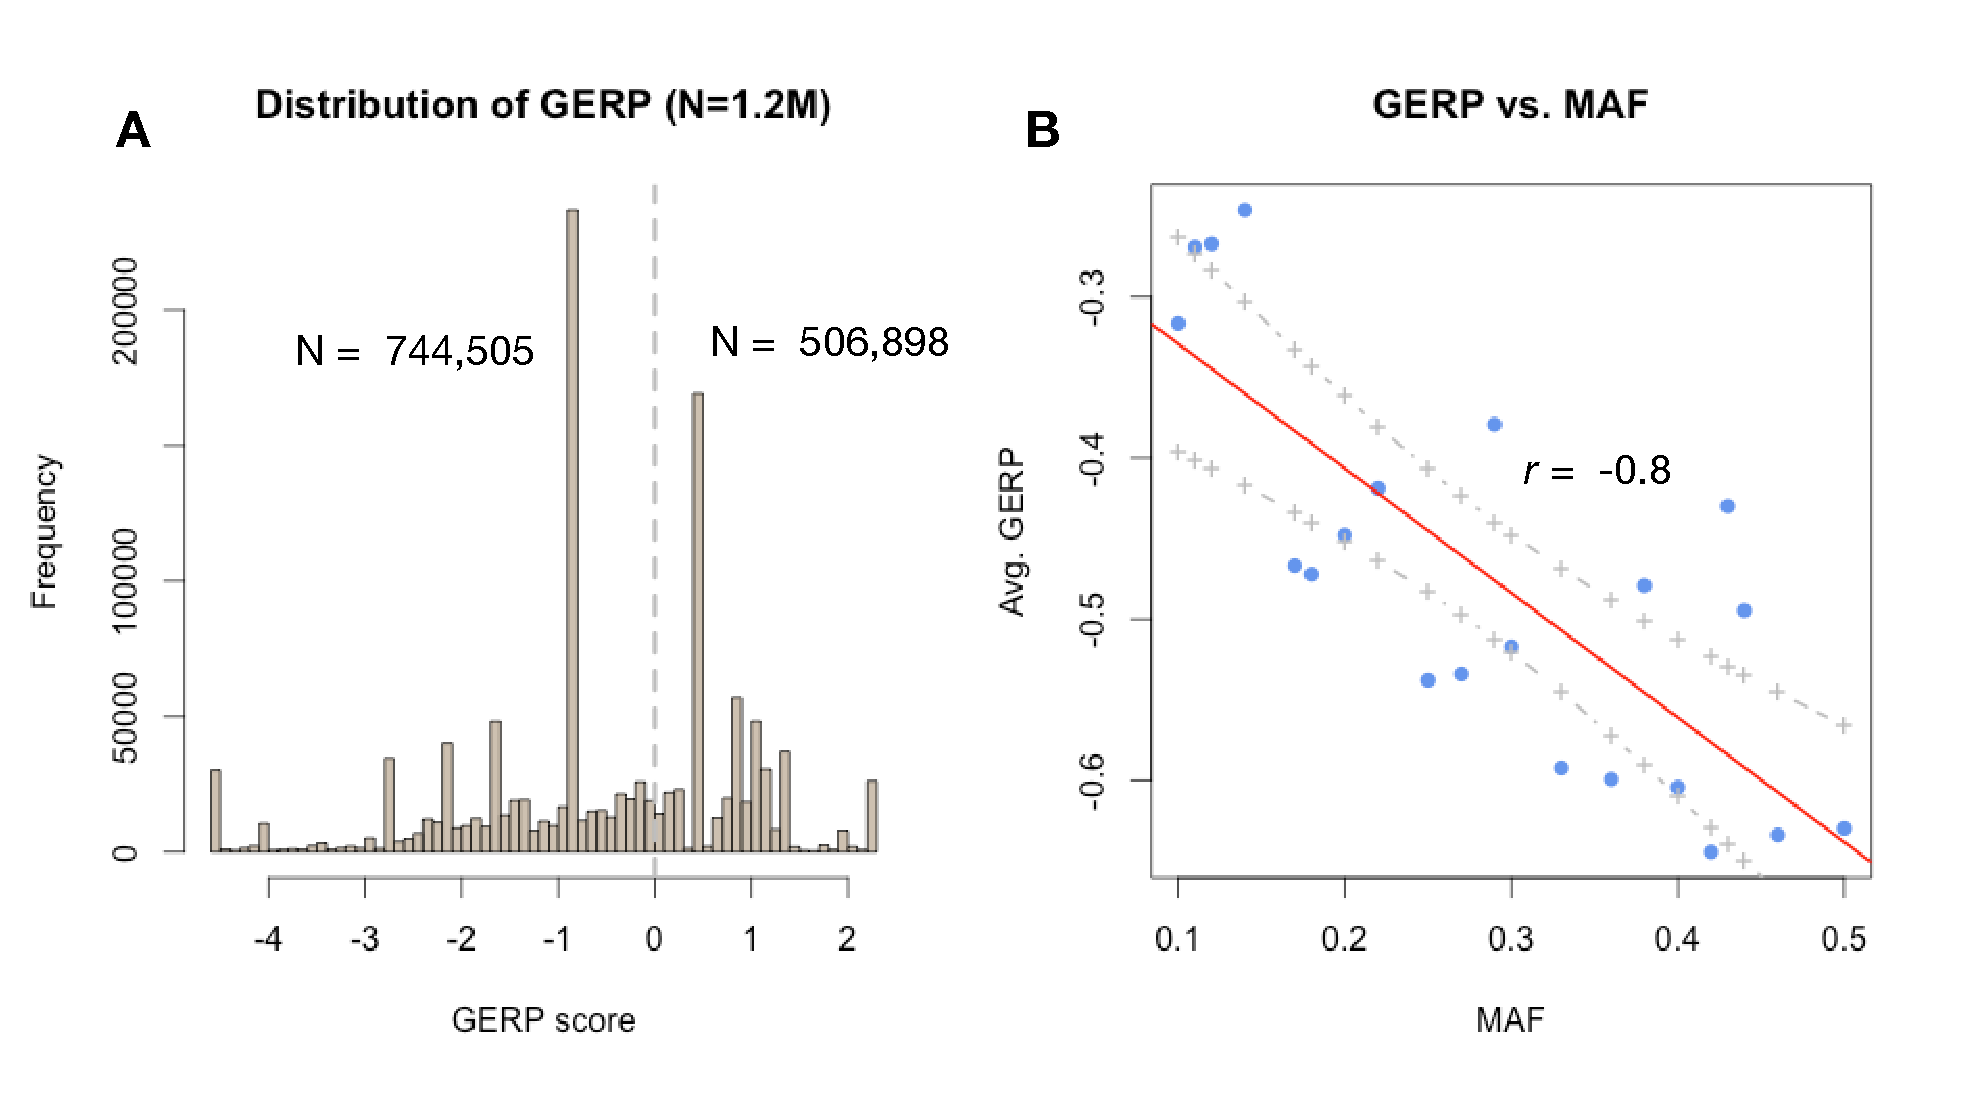
\includegraphics[width=\linewidth]{Figure_gerpmaf.pdf}
\caption{Distribution of GERP scores and relationship between GERP scores and MAFs. \textbf{(A)} Histogram of GERP scores extracted from $\sim$1.2 million sites where the GERP scores were available. \jri{1.2M is just the sites where GERP scores were available, correct?} \yang{yes, see edits} \textbf{(B)} Plot of average GERP scores in bins (bin size = 0.01) of minor allele frequency (MAF). The red and grey lines define the regression and its 95\% confidence interval.}
\label{fig:gerpmaf}
\end{figure}
%%%%%%%% ------------- %%%%%%%%%%%


\subsection*{Incorporatipn of GERP information improved prediction accuracies}

%where the haplotype was coded with the SNP conservation score as the explainatory variables. 
Genomic variants occurred at the evolutionary constraint sites were potentially deleterious. The phenotypic effects of these genetic loads and their contributions to heterosis become an interesting area to explore. However, the population size in this study is relative small and SNPs detected at sites containing high GERP scores are generally in low frequencies. The statistical power to detect the separate effects of these putative deleterious alleles becomes very low. To alleviate the statistical limitations, we conceived a haplotype-based approach for GS, which could add up individual effects of deleterious alleles in IBD blocks and estimate these IBD blocks simultaneously. To conduct the analysis, first of all, 55,000 IBD blocks were identified, which had an average size of 44,980 bp (ranged from 36 to 10,320,000 bp). IBD blocks having > 1-kb in size and containing > 1 deleterious alleles (SNPs at sites with GERP scores >0) were kept for further analysis. Secondly, the GERP scores of SNPs in an IBD block were summed under both additive and dominant models. Those summed GERP scores on IBD blocks were considered as the measurements of the conservation of the haplotypes. More details of this procedure were illustrated in Figure \ref{fig:gerpibd}.      

A Bayesian-based statistical method (BayesC) \citep{habier2011extension} was employed for model training. Using a 5-fold cross-validation approach, the prediction accuracies of the real data and cicularly shuffled data were compared. As shown in Figure \ref{fig:gerpall}, for traits \emph{per se}, prediction accuracies were significantly (FDR < 0.05) improved for ASI and PHT when incorporating GERP information in the IBD blocks under the additive model; prediction accuracy was significantly improved for ASI under the dominant model. For heterosis transformation traits (BPH), incorporation of GERP scores improved BPH of GY under the additive model and improved BPH of DTP, DTS and TW under the dominant model (Figure \ref{fig:gerpall} C and D, Supplementary table 3). In general, the average prediction accuracis were higher using the additive model (mean \emph{r} = 0.81 and 0.49 for traits \emph{per se} and BPH) than the dominant model (mean \emph{r} = 0.70 and 0.42). And the prediction accuracies decreased for predicting heterosis transformations (BPH) as compared to the predictions for traits \emph{per se}.

It was argued that SNPs in genic regions might have higher GERP scores than those in non-genic regions. The circular shuffling permutations may shift the high GERP scores to non-genic regions. If that is the case, the approach tended to weigh more on genic SNPs. To rule out this possibility, we elected SNPs with GERP scores >0 in genic regions only and did the circular shuffling to assign GERP scores to the same set of the selected SNPs. By doing this, the method will not take advantage of genomic positional information any more. Noted that in this study less number of SNPs was selected (N = 316, 983). Nevertheless, model prediction accuracies were significantly improved for traits \emph{per se} of GY under the additive model. For heterosis transformations, prediction accuracies were significantly improved for BPH of GY and PHT under the additive model and the prediction accuracy was significantly improved for pBPH of GY (Figure \ref{fig:genicsnp} and Table S4).   


%%%%%%%% ----- BEAN PLOT using all GERP SNPs-------- %%%%%%%%%%%
\begin{figure}[htbp]
\centering
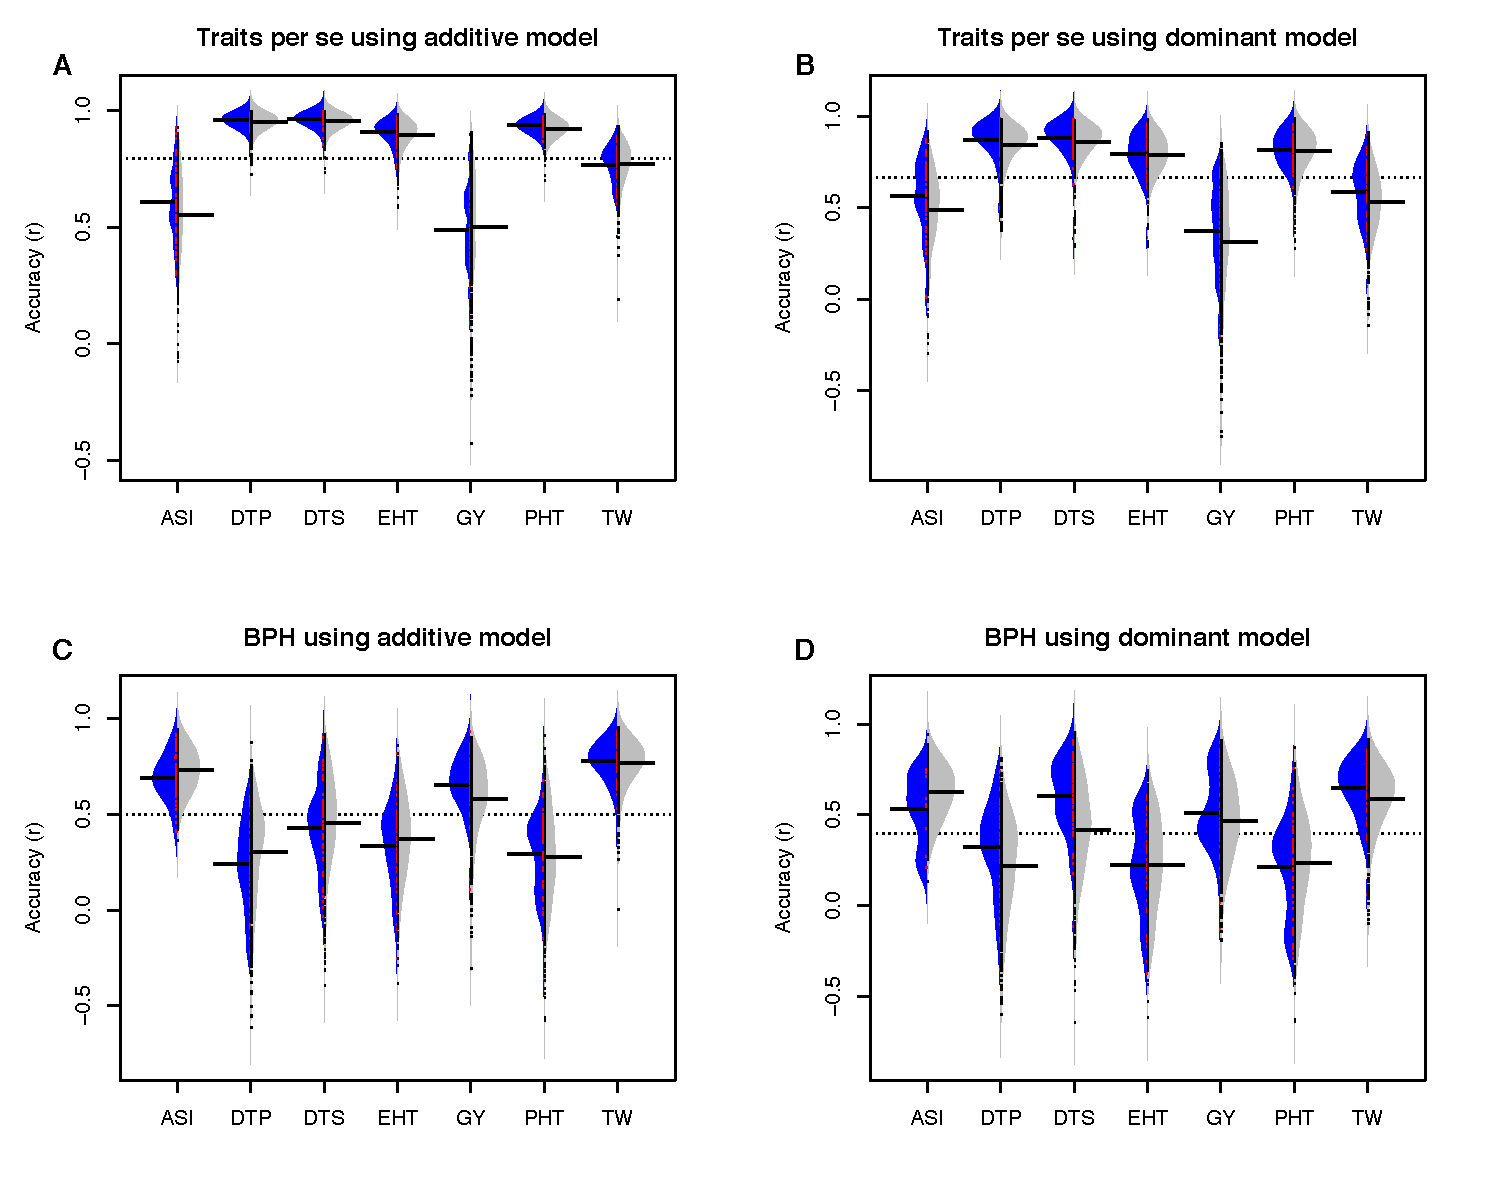
\includegraphics[width=\linewidth]{Figure_gerpall.pdf}
\caption{Beanplots of cross-validation accuracies using SNPs with positive GERP score. Cross-validation experiments were conducted using selected SNPs and circular shuffled data from the same set of SNPs for traits \emph{per se} (\textbf{A, B}), BPH (\textbf{C, D}) and pBPH (\textbf{E, F}) under additive (\textbf{A, C, E}) and dominant (\textbf{B, D, F}) models. Accuraries from the real data were plotted on the left side of the bean (blue) and permutation results plotted on the right (grey). Horizotal bars on beans indicate mean accuracies. The grey dashed lines indicate the overall average accuracies. Stars indicate significantly improved cross-validation accuracies with FDR < 0.05.}
\label{fig:gerpall}
\end{figure}
%%%%%%%% ------------- %%%%%%%%%%%


\subsection*{Posterior phenotypic variance explained and model comparisons}

To learn why the prediction performace varied among traits \emph{per se} and heterosis transformations, we obtained the posterior variance explained by our models using the complete set of data. As shown in Figure \ref{fig:h2}, additive models explained more phenotypic variance for traits \emph{per se} of DTP, DTS, EHT and PHT; but explained less phenotypic variance for heterosis transformations (BPH) of ASI, GY and TW. On the contrary, lager proportions of the phenotypic variance could be explained by the dominant models for heterosis transformations (BPH) of ASI, GY and TW. For the GY in particular, 50\% of the heterosis could be explained by dominant model.   

Heterosis transformations were largely determined by the accuracies of the parental phenotypes. To take the uncertainty of the parental phenotypes into consideration, we estimated the combining abilities from the hybrid population itself to investigate which modes of inheritance perform better than the null models. We extracted the breeding values estimated with both additive and dominant models using the genome-wide IBD blocks incorporated with the GERP scores. Consistent with above analysis, IBD blocks coded with dominant mode of inheritance significantly (equation \ref{eq:refname1} vs. equation \ref{eq:refname2}, ANOVA \emph{P} value < 0.05 ) improved model fitting for ASI and GY. We also compared model \ref{eq:refname3} and model \ref{eq:refname4}, ANOVA results indicated that \ref{eq:refname4} performed almost as good as \ref{eq:refname3}, indicating that specific combining ability captured most of the parental interactions and the current method could not detect higher order of interactions. 

\begin{equation}
Y_{ij} = \mu + GCA_{i} + GCA_{j} + \varepsilon
\label{eq:refname1}
\end{equation}
\begin{equation}
Y_{ij} = \mu + GCA_{i} + GCA_{j} +  G_{ij} + \varepsilon
\label{eq:refname2}
\end{equation}
\begin{equation}
Y_{ij} = \mu + GCA_{i} + GCA_{j} + SCA_{ij} + \varepsilon
\label{eq:refname3}
\end{equation}
\begin{equation}
Y_{ij} = \mu + GCA_{i} + GCA_{j} + SCA_{ij} + G_{ij} + \varepsilon
\label{eq:refname4}
\end{equation}
where 
$Y_{ij}$ is the BLUE value of the hybrid crossed between the $i^{th}$ inbred and $j^{th}$ inbred; 
$\mu$, the overall mean; 
$GCA_{i}$, the general combining ability of the $i^{th}$ inbred;
$GCA_{j}$, the general combining ability of the $j^{th}$ inbred;
$SCA_{ij}$, the specific combining ability of between the $i^{th}$ and $j^{th}$ inbreds;
$\varepsilon$, the model residuals.

%%%%%%%% ----- h2 plots-------- %%%%%%%%%%%
\begin{figure}[htbp]
\centering
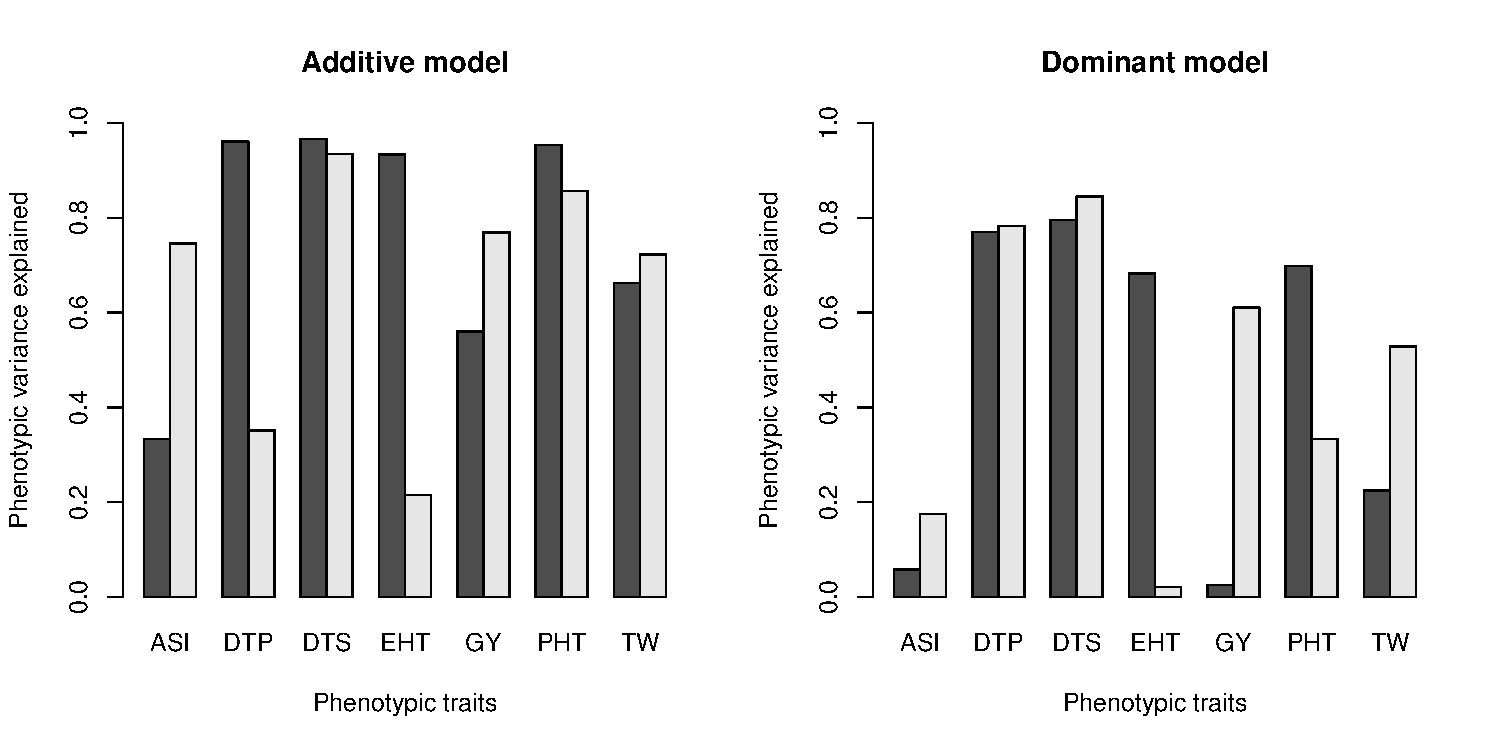
\includegraphics[width=\linewidth]{Figure_h2.pdf}
\caption{Barplots of the phenotypic variance explained by IBD blocks incorporated with GERP scores.}
\label{fig:h2}
\end{figure}
%%%%%%%% ------------- %%%%%%%%%%%


%%%%%%%%%%%%%%%%%%%% DISCUSSION %%%%%%%%%%%%%%%%%%%%%%%%%%%%%%%
\section*{Discussion}

\begin{itemize}
  \item do we support deleterious model of Mezmouk et al.? \yang{yes}
  \item how do results match with heritability and heterosis? \yang{and mode of inheritance}
  \item Indication for breeding? genomic selection using GERP and other annotation information. 
\end{itemize}


In this study, more than 500,000 deleterious SNPs were identified in elite maize lines. On average, each elite inbred line carries about 100,000 deleterious SNPs (GERP > 0). In the population, however, majority of these deleterious mutations were maintained in a low frequency, which consistent with previous observation \citep{rodgers2015recombination}. The large number of deleterious alleles make it hard to be completely purged through breeding efforts. In practice, part of the genetic loads could be released in F1 hybrids by combining appropriate inbred lines (from pre-defined heterotic groups) to complement deleterious alleles. Indeed, results in this study shown that prediction accuracies were higher for yield heterosis using deleterious SNPs than permuted ones. Because we weighted SNPs with their conservation score in GS model, the improved accuracies could be attributed to deleteriousness of SNP variants. Therefore, it provided evidence of complementation of deleterious alleles for heterosis \citex{}. Note that thousands of deleterious alleles may be involved in the complementation, and most of which may have minor effects. Their effects could not be easily detected by traditional QTL or GWAS \citex{}.

To test hypothesis, we developed a GS pipeline, which incorporated evolutionary conservation information in the GS model. As the genotyping cost keeps declining, GS tends to replace marker assistant selection (MAS) \citex{} in plant breeding \citex{}. Researchers developed a series of statistical approaches to improve the efficiency of GS model \citex{}, however, none of the existing approaches have taken prior biological information into consideration. It is known that SNP variations would have varied impacts depending on their genomic position (e.g. ) \citex{}, biological function (e.g. transcription binding sites) and evolutionary conservation. The incorporation of GERP information under the Bayesian framework developed in this study is the first step towarding more meaningful models for further GS.     

It was not surprised that the current models did not increase the prediction accuacies equally well for traits \emph{per se} and their heterosis transformations. Genetic arachitectures of different phenotypic traits varied in maize and other crop species, e.g., flowering time of maize was determined by many small effect additive loci \citex{} and rice yield was determined by many dominant loci \citex{}. We observed additive model increased the prediction accuacies for trait \emph{per se} of ASI and dominant model increased the prediction accuacies for trait \emph{per se} of GY. Because under current models, we simply assume phenotypic traits were determined by complete additive or complete dominant effects. Traits with mixture effects of additive and dominant loci may fail to be predicted. In addition, the population size was relative small in the model training, we may not have enough power to predict traits with low heritability. 

% Paritcally, with dominant model, up to 20\% of the phenotypic variance could be explained for the heterosis traits. Theoritically, BPH transformation subtracts the joint effects of the additive and dominant alleles in the best parents as residule, the substantial variance of these redidules explained by the additive or dominant models in our studies indicated that genetic components controlling for heterosis might in linked state.  

% How to explain the prediction difference?  
% The variation of the prediction accuacies were relative large in this study. First of all, broad sense heritability of the traits are different. Second, from the simulation we learned that different traits may controlled by different proportion of additive, dominant and even recessive gene actions. Our naive model only built the pure additive and pure dominant effects in. For the more complicated cases, the models may not work very well.



%%%%%%%%%%%%%%%%%%%%%%%%%%%%%%%%%%%%%%%%%%%%%%%%%%%%%%%%%%%%%%%

\clearpage
\bibliography{Diallel}



\onecolumn
%Figure
%----------------------------------------
% SUPPLEMENTARY FIGURES
%----------------------------------------
\pagebreak
\beginsupplement

\section*{Supporting Information}

% \section*{Supporting Table}:
\begin{center}\vspace{1cm}

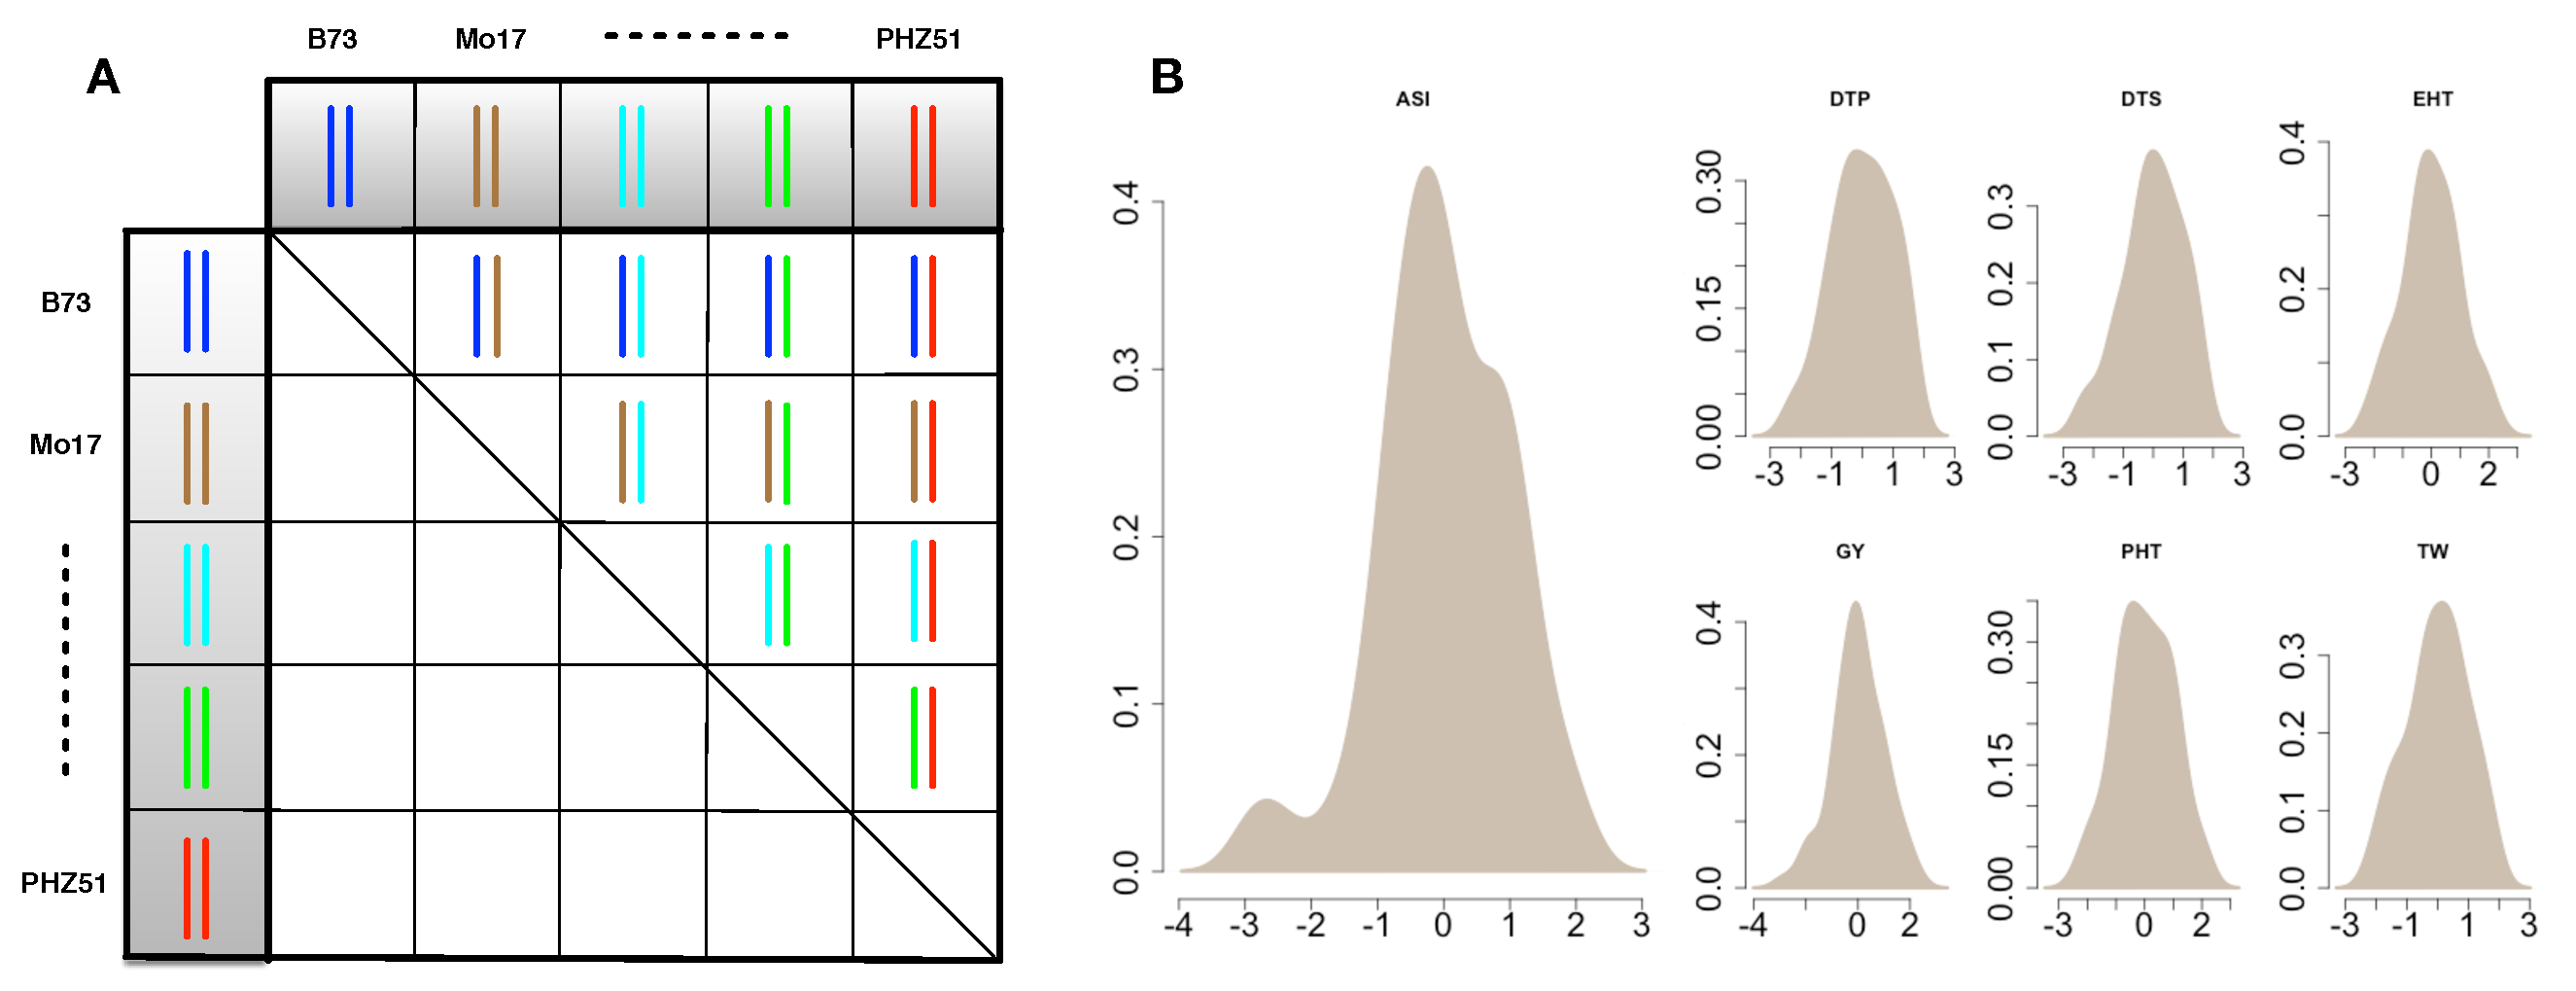
\includegraphics[width=0.8\linewidth]{SFig_pvp.pdf}
\captionof{figure}
{\color{black} \textbf{Diallel experimental design and distribution of phenotypic data.}
\textbf{(A)} Twelve maize inbred lines were selected and crossed in a partial diallel. \jri{do we need to modify this diagram now that we now reciprocal crosses were pooled?} \textbf{(B)} Density plots of the phenotypic distributions.
}
\label{fig:pvp-pheno}
\end{center}\vspace{1cm}

%%%%%%%% ----- pBPH-------- %%%%%%%%%%%
\begin{figure}[htbp]
\centering
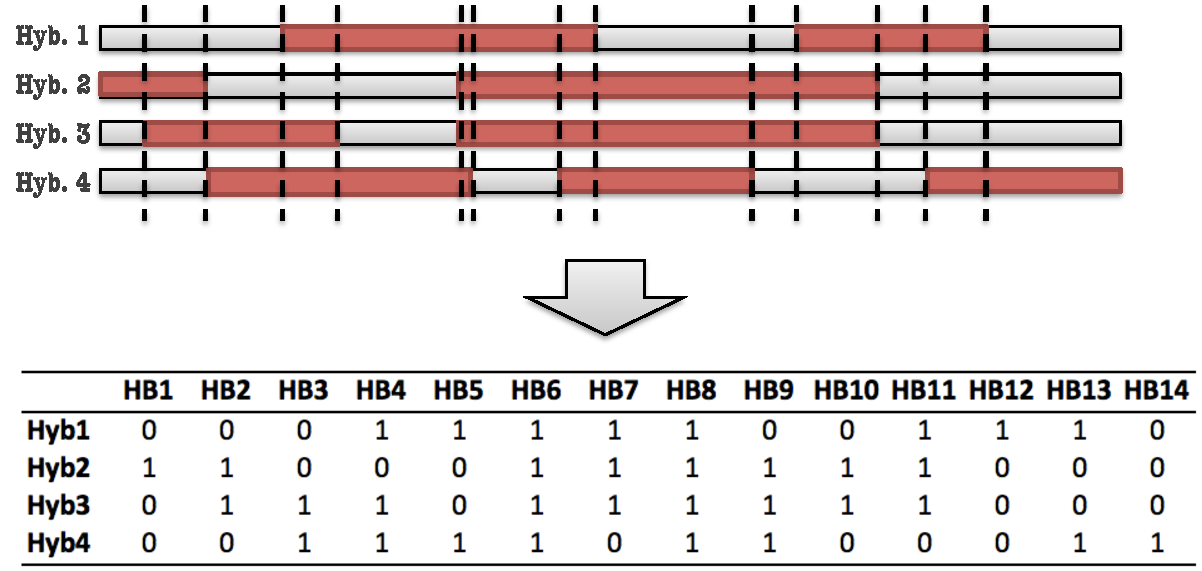
\includegraphics[width=\linewidth]{SFig_define_IBD.pdf}
\caption{Haplotype block identification using an IBD approach. In the upper panel, regions in red are IBD blocks identified by pairwise comparison of the two parental lines of a hybrid. The vertical dashed lines define haplotype blocks. In the lower panel, hybrid genotypes at each block are coded as heterozygotes (0) or homozygotes (1).}
\label{fig:defineibd}
\end{figure}
%%%%%%%% ------------- %%%%%%%%%%%



%%%%%%%% ----- pBPH-------- %%%%%%%%%%%
\begin{figure}[htbp]
\centering
\includegraphics[width=\linewidth]{SFig_pBPH.pdf}
\caption{Boxplot of  percent best parent heterosis (pBPH). In the plot, ASI was calculated using pBPHmin and the other six traits were calculated using pBPHmax.}
\label{fig:pBPH}
\end{figure}
%%%%%%%% ------------- %%%%%%%%%%%

%%%%%%%% ----- GERP dis1m -------- %%%%%%%%%%%
\begin{figure}[htbp]
\centering
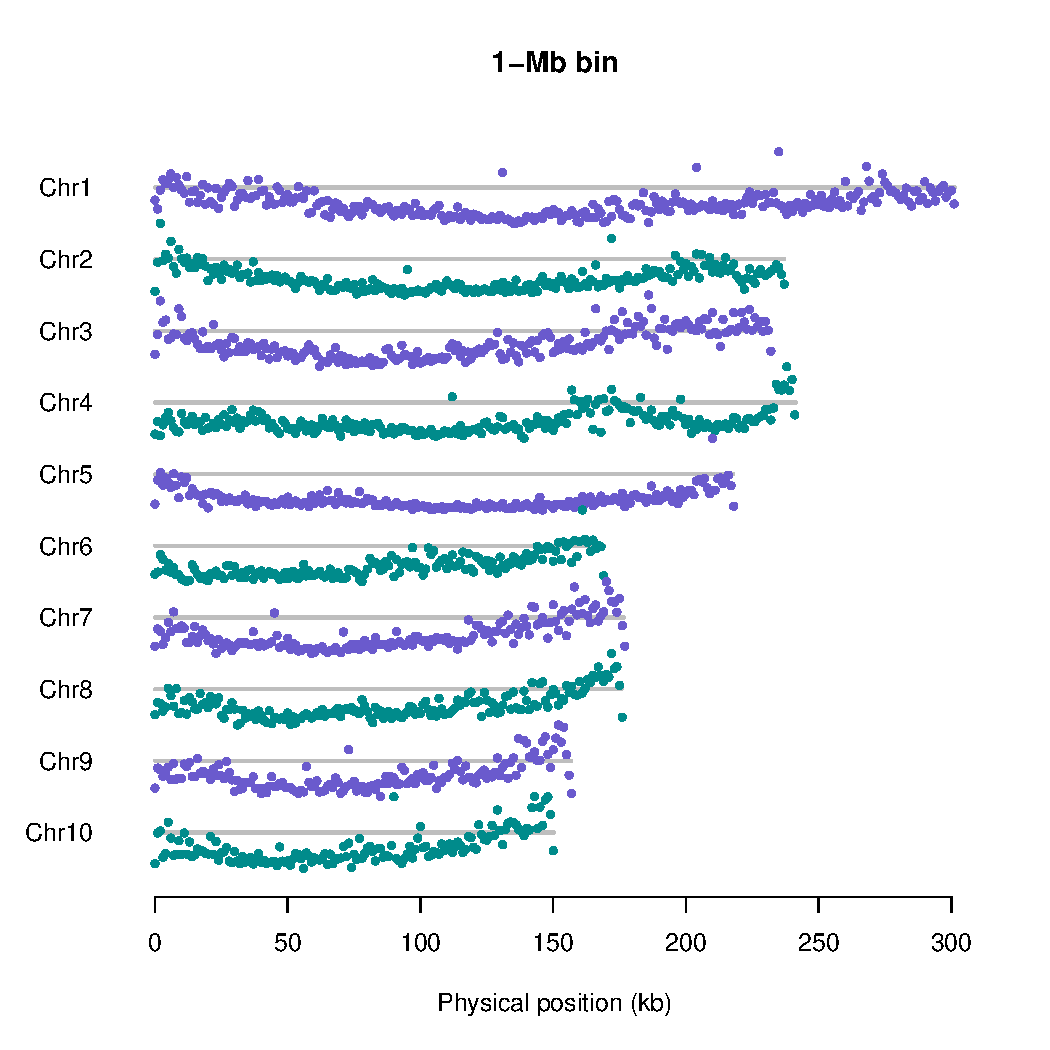
\includegraphics[width=\linewidth]{SFig_gerp_dis1m.pdf}
\caption{GERP score distribution across the genome. Shown are mean GERP scores in a 1-Mb bin region.}
\label{fig:dis1m}
\end{figure}
%%%%%%%% ------------- %%%%%%%%%%%

%%%%%%%% ----- GERP IBD diagram -------- %%%%%%%%%%%
\begin{figure}[h]
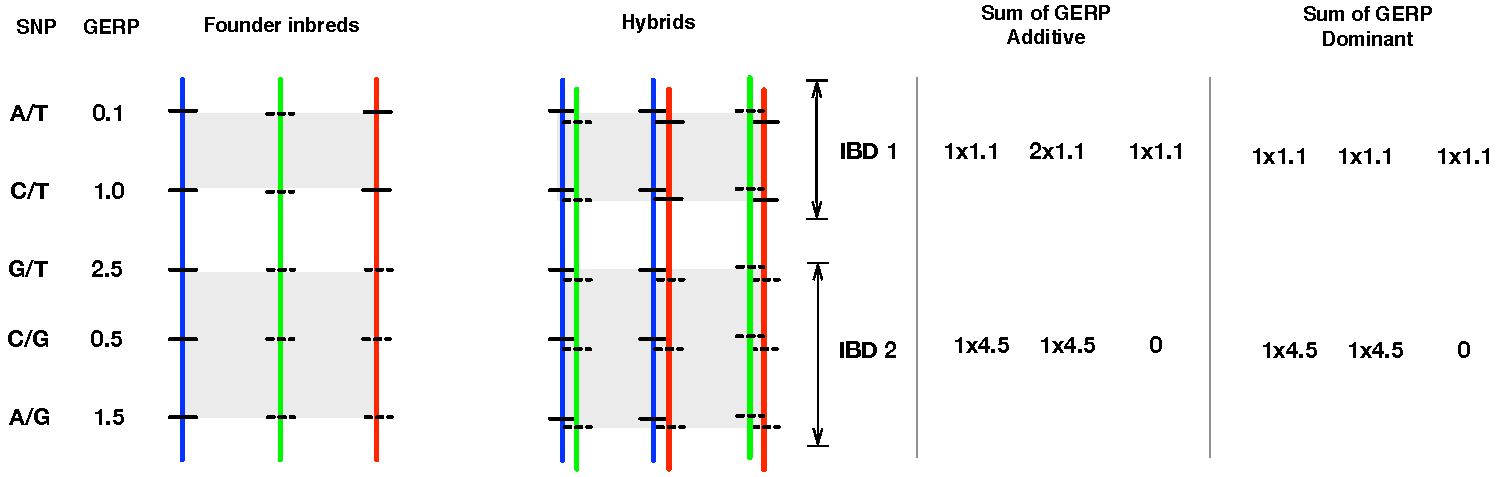
\includegraphics[width=0.9\textwidth]{SFig_gerpIBD.pdf}
\caption{
\textbf{Incoporation of conservation information into IBD blocks.}
Regions of the genome that are identical by descent (IBD) among the 12 inbreds were identified using Beagle \citep{Browning2009}.  The GERP scores of SNPs in an IBD block were summed under both additive and dominant models. For a particular SNP with GERP score $g$, the homozygous non-reference genotype was assigned a value of $2g$, the heterozygote assigned a value of $g$, and the reference homozygote a value of 0.  Under the dominant model, both the heterozygote and the non-reference homozygote were assigned a value of $g$, with the reference homozygote again assigned a value of 0.}
\label{fig:gerpibd}
\end{figure}
%%%%%%%% ------------- %%%%%%%%%%%

%%%%%%%% ----- BEANPLOT-------- %%%%%%%%%%%
\begin{figure}[htbp]
\centering
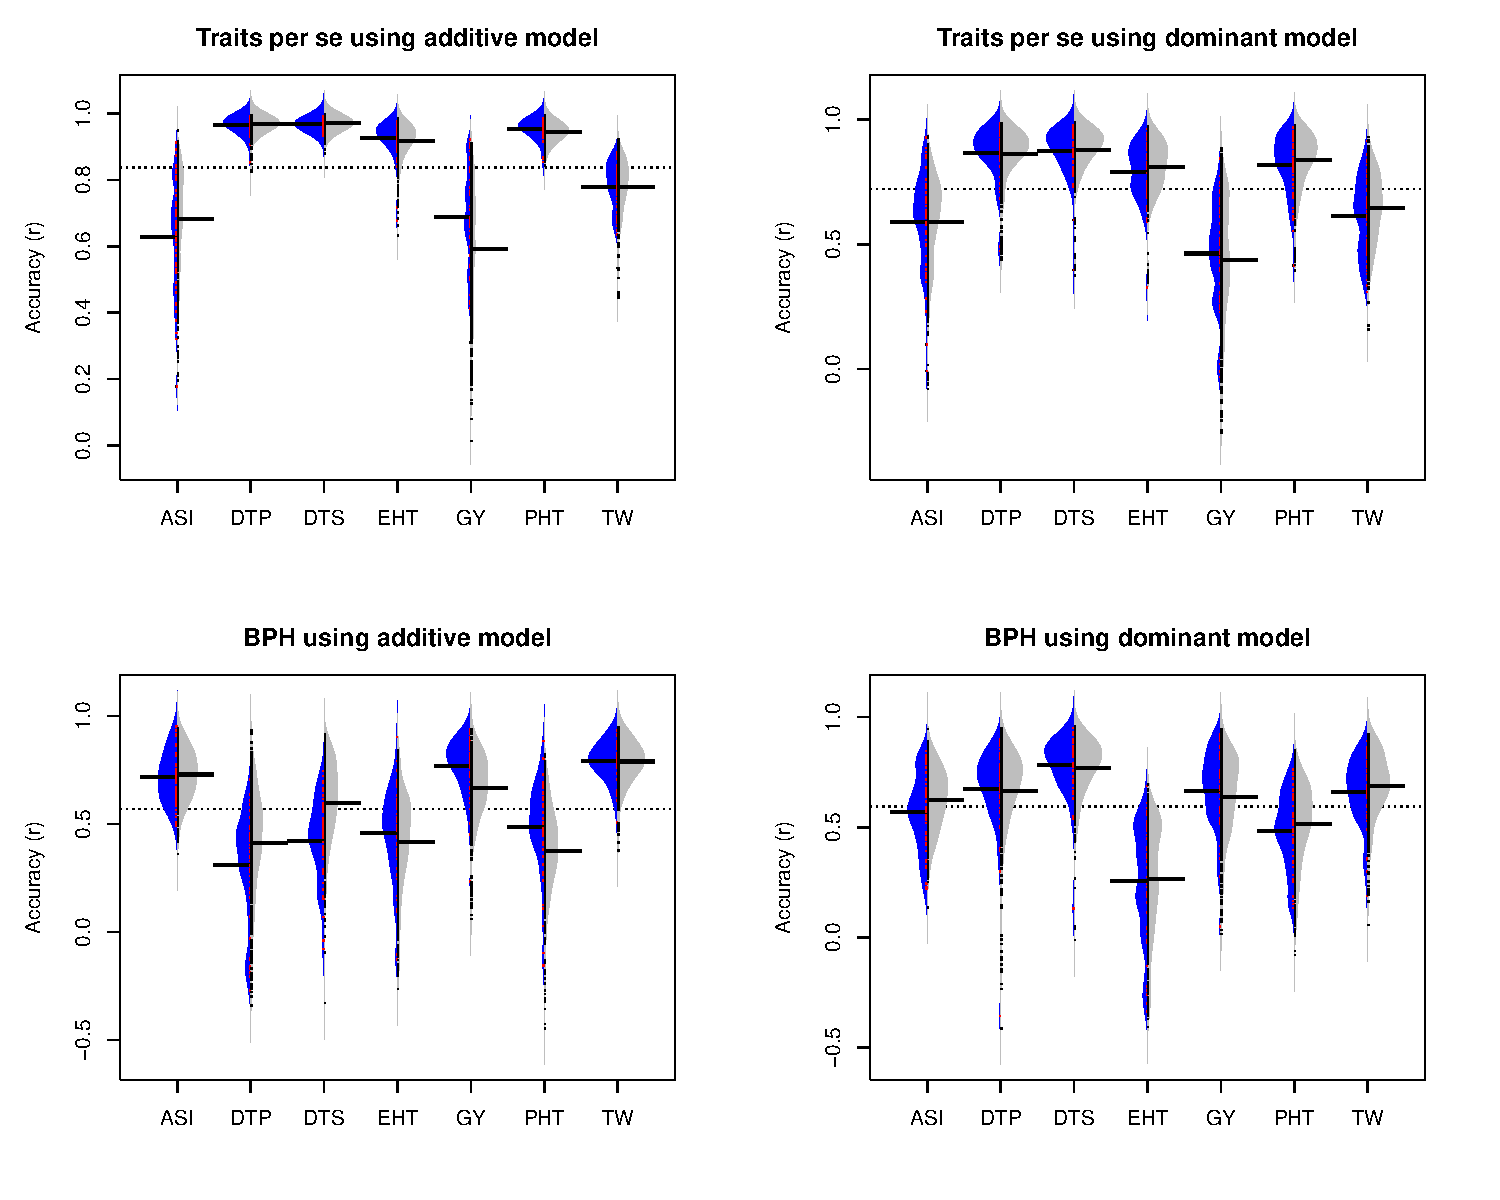
\includegraphics[width=\linewidth]{SFig_genicsnp.pdf}
\caption{Cross-validation accuracies using genic SNPs. Cross-validation experiments were conducted using genic SNPs and compared to circular-shuffled data for traits \emph{per se} (\textbf{A, B}) and pBPH (\textbf{C, D}) under additive (\textbf{A, C}) and dominant (\textbf{B, D}) models. Distirbutions show accuracty of prediction from real data (blue) and permutations (grey), with horizontal bars to indicate mean accuracy.  Stars indicate significantly higher cross-validation accuracy for the real data.  The average accuracy across all traits is shown with the grey dotted line. }
\label{fig:genicsnp}
\end{figure}
%%%%%%%% ------------- %%%%%%%%%%%

\end{document}